\section{Generalized Minimum Variance Control}

The primary limitations of Minimum Variance Control are:
\begin{itemize}
    \item It can only be applied to minimum phase systems.
    \item There is no moderation of the effort and intensity of the control action $u(t)$. 
    \item t lacks the capability to design a specific behavior or relationship between $y^{0}(t)$ and $y(t)$. 
\end{itemize}
To address these limitations, Generalized Minimum Variance Control extends Minimum Variance Control.

\subsection{Performance indexes comparison}
For Minimum Variance Control, the performance index is:
\[J=\mathbb{E}\left[\left(y(t)-y^{0}(t)\right)^2\right]\]
However, for Generalized Minimum Variance Control, the performance index is more comprehensive:
\[J=\mathbb{E}\left[\left(y(t)-P(z)y^{0}(t)+Q(z)u(t)\right)^2\right]\]
Here, the additional term $Q(z)u(t)$ penalizes the usage of control effort, and $P(z)$ establishes a reference model between $y^{0}(t)$ and $y(t)$. 
It's noteworthy that Generalized Minimum Variance Control reduces to simple Minimum Variance Control when $P(z)=1$ and $Q(z)=0$. 

\paragraph*{Reference model matrix}
The matrix $P(z)$ serves as the reference model for the closed-loop system's desired behavior. 
In general, we envision the ideal scenario as:
\begin{figure}[H]
    \centering
    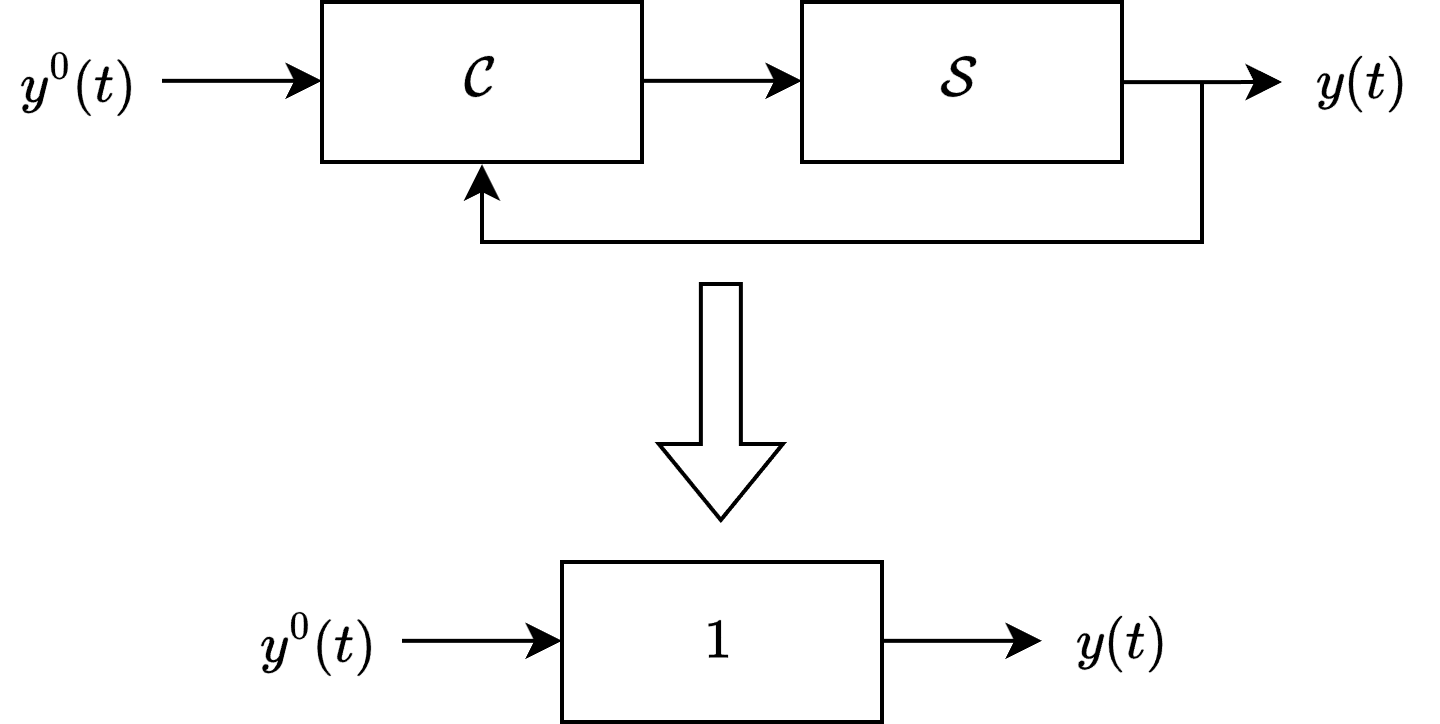
\includegraphics[width=0.5\linewidth]{images/p.png}
    \caption{Ideal scenario}
\end{figure}
It's important to note that in some systems, the optimal behavior isn't always achieved when $P(z)=1$. 
In such cases, a low-pass filter $P(z)$ might be employed to establish a new target for the closed loop.

\begin{example}
    Given the ARMAX system:
    \[y(t)=\dfrac{2}{3}y(t-1)+u(t-1)+\dfrac{1}{3}u(t-2)+3e(t-2)\qquad e(t)\sim WN(0,1)\]
    We aim to design the Minimum Variance Control for this system.
    
    The system's transfer function is:
    \[y(t)=\dfrac{1+\frac{1}{3}z^{-1}}{1-\frac{2}{3}z^{-1}}u(t-1)+\dfrac{3}{1-\frac{2}{3}z^{-1}}e(t-2)\]
    Here's how we proceed:
    \begin{enumerate}
        \item Assumption check:
            \begin{itemize}
                \item The system is minimum phase since $\frac{1}{3}$ lies inside the unit circle.
                \item We need to find the canonical representation of the system, given by 
                    \[\dfrac{1}{1-\frac{2}{3}z^{-1}}\eta(t-2) \qquad \eta(t)\sim WN(0,9)\]
            \end{itemize}
        \item We apply the Minimum Variance Control formula to the canonical representation of the ARMAX:
            \[y(t)=\dfrac{1+\frac{1}{3}z^{-1}}{1-\frac{2}{3}z^{-1}}u(t-1)+\dfrac{1}{1-\frac{2}{3}z^{-1}}\eta(t-2)\]
            After performing one step of long division, we obtain $E(z)=1$, and $R(z)=\frac{2}{3}z^{-1}$. 
            The Minimum Variance Control system is then implemented according to the obtained controller structure.
            \begin{figure}[H]
                \centering
                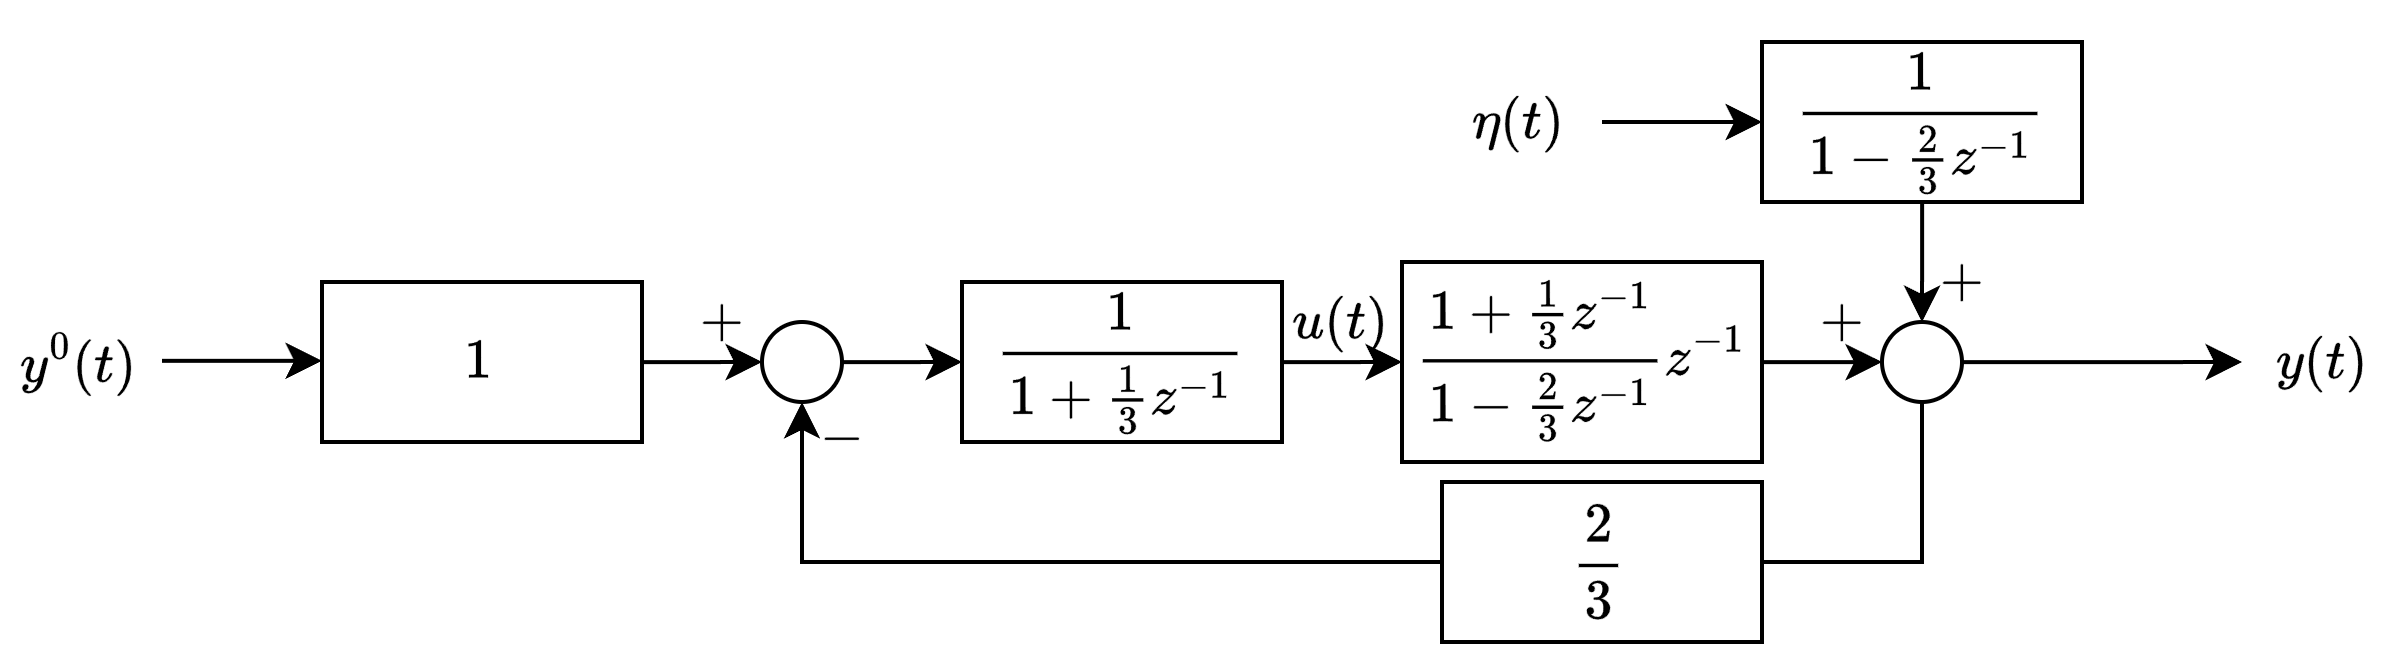
\includegraphics[width=0.75\linewidth]{images/mvc.png}
            \end{figure}
    \end{enumerate}
\end{example}